\section{Indledning}
Projektets omhandler behandling af lyd, objektorienteret programmering samt en brug af datakommunikation og softwareudvikling.

To bærbare computere skal kommunikere med hinanden ved hjælp af lyd, hvortil der blev udleveret 2 sæt mikrofoner og højtalere.
Der skal bruges DTMF toner til kommunikationen. Det er de tastetoner der er på telefoner.\\%Måske skrive dette et andet sted.
DTMF står for Dual Tone Multiple Frequency, hvilket betyder at der ligger to toner oven i hinanden med forskellig frekvens, f.eks taste tone 1, er 679 Hz og 1209 Hz

\begin{figure}[h]
\centering
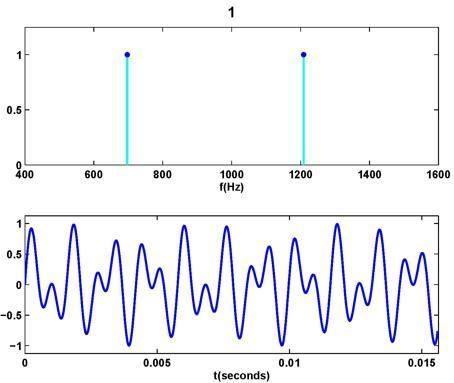
\includegraphics[scale=0.5]{Billeder/DTMF1.JPG}
\caption{DTMF tone 1}
\label{fig:DTMF1}
\end{figure}

Projektet skal skrives i programmeringssproget C++ som er et objektorienteret sprog.
samtidig skal software arkitekturen være lagdelt, eksempelvis et fysisk lag og et datalink lag.

Programmet som udvikles skal udføre noget meningsfyldt, så som en chat-klient.